\section{German}
\newcommand\arrow{$\,\Rightarrow\,$ }

A summary of the German language syntax

\subsection{Nomenclature}
verben:\\
Tempus = Tense = präsens / präteritum\dots\\
Modi = Indikativ / Konjuktiv I \& II / Imperativ\\
Genus = Aktiv / Passiv\\
Verbartes = Hilfsveben / Modalverb / Vollverben

\subsection{Verbs}

Verbs are sometimes used

\subsubsection{Tenses}

% TODO: al porta in nomenclature?
HV = Hilfsveben = Sein / Haben / Werden \\
MV = Modalverb = dürfen / können / mögen / müssen / sollen / wollen \\
Vollverben = verbi nurmai \\
\\
Partizip II = gespielt \\
\\
Präsens = Verb in präsens \\
Präteritum = Verb in präteritum \\
Perfekt = HV präsens + Partizip II \\
Plusquamperfekt = HV präteritum + Partip II \\
Futur I = Werden + Infinitv \\
Futur II = Werden + Partizip II + haben/sein \\

Beim Hauptsatz + nebesatz gilt: Präteritum + Plusquamperfekt / Präsens + Perfekt

\begin{center}
\begin{tabular}{|c|c|c|c|c|c|c|}
    \textbf{} & \textbf{Präsens} & \textbf{Präteritum} & \textbf{Perfekt} & \textbf{Plusquamperfekt} & \textbf{Futur I} & \textbf{Futur II} \\
    \textbf{Ich} & spiel\textbf{e} & spiel\textbf{te} & habe gespiel\textbf{t} & hatte gespiel\textbf{t} & werde spiel\textbf{en} & werde gespiel\textbf{t} haben \\
    \textbf{Du} & spiel\textbf{st} & spiel\textbf{test} & hast gespiel\textbf{t} & hattest gespiel\textbf{t} & wirst spiel\textbf{en} & wirst gespiel\textbf{t} haben \\
    \textbf{Er/Sie/Es} & spiel\textbf{t} & spiel\textbf{te} & hat gespiel\textbf{t} & hatte gespiel\textbf{t} & wird spiel\textbf{en} & wird gespiel\textbf{t} haben \\
    \textbf{Wir} & spiel\textbf{en} & spiel\textbf{ten} & haben gespiel\textbf{t} & hatten gespiel\textbf{t} & werden spiel\textbf{en} & werden gespiel\textbf{t} haben \\
    \textbf{Ihr} & spiel\textbf{t} & spiel\textbf{tet} & habt gespiel\textbf{t} & hattet gespiel\textbf{t} & werdet spiel\textbf{en} & werdet gespiel\textbf{t} haben \\
    \textbf{Sie/Sie} & spiel\textbf{en} & spiel\textbf{ten} & haben gespiel\textbf{t} & hatten gespiel\textbf{t} & werden spiel\textbf{en} & werden gespiel\textbf{t} haben \\
\end{tabular}
\end{center}

\subsubsection{Modi}

\subsection{Satzglieder}

\href{run:./includes/german/GBC/GBC_Satzglieder_2022.pdf}{GBC\_Satzglieder\_2022.pdf}

\subsubsection{Prädikat}

Prädikat = Verb (a piece may be detached)\\
\\
Eifach \arrow Der Löwe \textbf{brüllt}.\\
Imperativ \arrow \textbf{Lauf} schneller.\\
Verbzusatz \arrow Er \textbf{wandete} sich \textbf{ab}.\\
MV + Verb \arrow Er \textbf{wollte} besser \textbf{lernen}.\\
\\
Verneinung \arrow Ich \textbf{habe} das \textbf{nicht gekauft}.\\
Reflexivpronomen \arrow Er \textbf{setz sich} auf die Bank.\\

\subsubsection{Subject}
\newcommand\textover[2]{$\overbrace{\text{#1}}^{\text{#2}}$}

The only one that is in Nominativ.\\
Person un numeros of the Subject change the conjugation of the predicate.\\
\\
GN = Gleichsetzungsnominativ \arrow \textover{Er}{Subject} \textover{ist / Wird / Heisst / Bleibt}{Predikat} \textover{Student}{GN}\\

\subsubsection{Objekt}

AO = Akkusativobject = who or what? \arrow Ich lese \textbf{ein Buch}.\\
DO = Dativobject = wem / whom? \arrow Er gratuliere \textbf{ihr}.\\
GO = Genitivobject = wessen / whose? \arrow Sie bedarf \textbf{seiner Hilfe}.\\
PO = Präpositionalobject = Präposition + who / whom \arrow Ich denke \textbf{an dich}\\
\\
Akkisativ => - für - um - durch - gegen - ohne
Dativ => aus - bei - mit - nach - seit - zu - von

\subsubsection{Adverbial}

Adverbials describe the circumstances

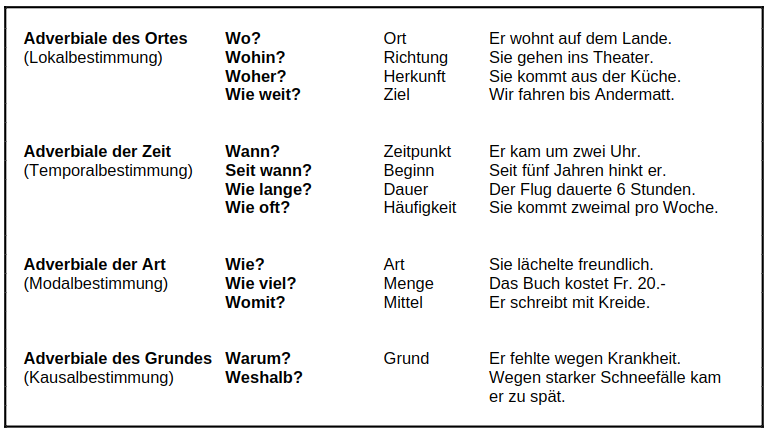
\includegraphics[width=\textwidth]{./german/imgs/adverbial.png}

\subsubsection{Attributes}
Das Attribut ist kein Satzglied.\\

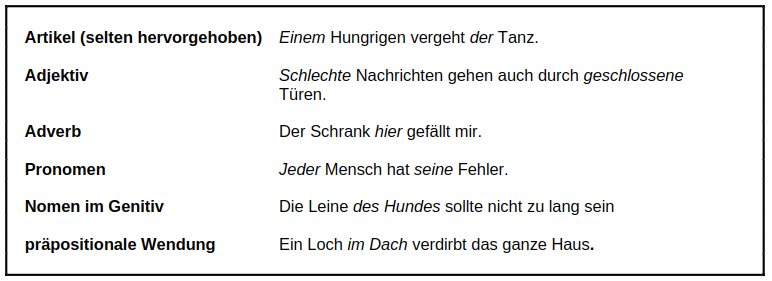
\includegraphics[width=\textwidth]{./german/imgs/attribut.png}

\subsubsection{Apposition}

Die apposition ist kein Satzglied.\\
Es erläutert die Nomen näher und steht im gleichen Fal.\\
\\
Martin, \textbf{unser Torwart}, ist leider krank.\\
Johannes Gutenberg, \textbf{der Erfinder des Buchdrucks}, lebte in Mainz.


\subsection{Syntax}

\href{run:./includes/german/GBC/GBC_Syntax_2022.pdf}{GBC\_Syntax\_2022.pdf}

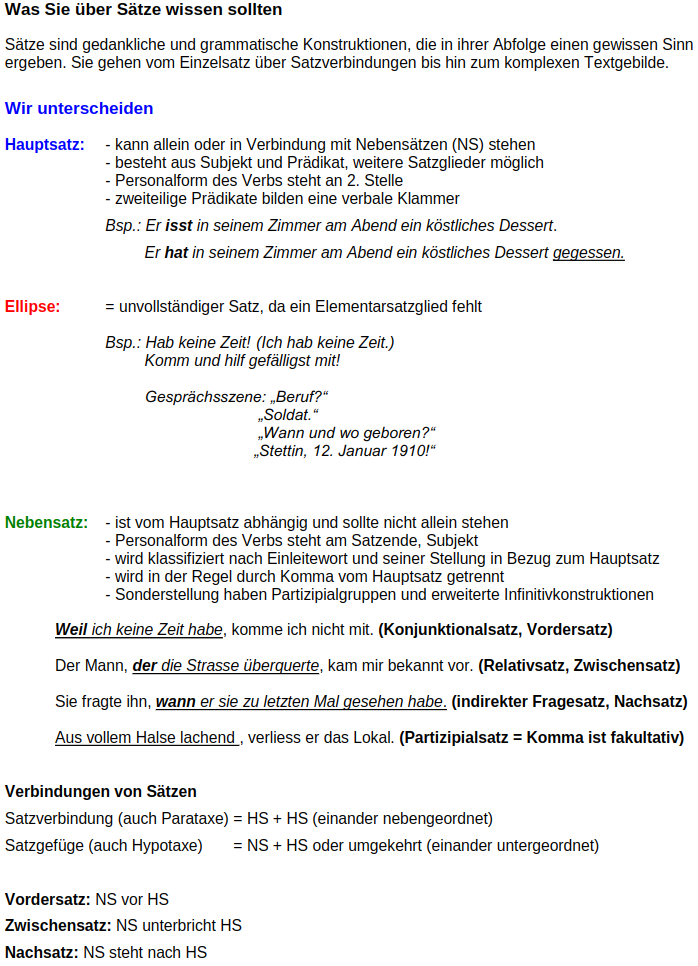
\includegraphics[width=\textwidth]{./german/imgs/satze.png}

\subsubsection{Satzarten}
Eine Teilsatz ist eien einzelne HS oder NS.

\begin{description}
    \item[Fragment/Ellipse:] fehlt etwas \arrow Wegen Krankheit geschlossen.
    \item[HS:] Der einfache Satz \arrow Wir haben wegen Krankheit geschlossen.
    \item[SV:] Satzverbindung = HS + HS \arrow Die Temperatur ist gefallen, und es schneit bereits.
    \item[SG:] Satzgefüge = NS + HS
    \begin{description}
        \item[Vordersatz:] NS + HS \arrow Weil die Temperaturen gefallen sind, schneit es jetzt.
        % \item[Zwischensatz] HS + NS + HS \arrow Ich lese, sobald ich zu Hause bin, meine Zeitung.
        \item[Zwischensatz:] HS + NS + HS \arrow Es schneidet, weil die Temperaturen gefallen sind, jetz.
        \item[Nachsatz:] HS + NS \arrow Es schneidet jetz, weil die Temperaturen gefallen sind.
    \end{description}
    \item[Zusammengezogene:] NS fehlt etwas \arrow Die Blumen machen den Garten, nicht der Zaun.
\end{description}

\subsubsection{Nebensatzarten}

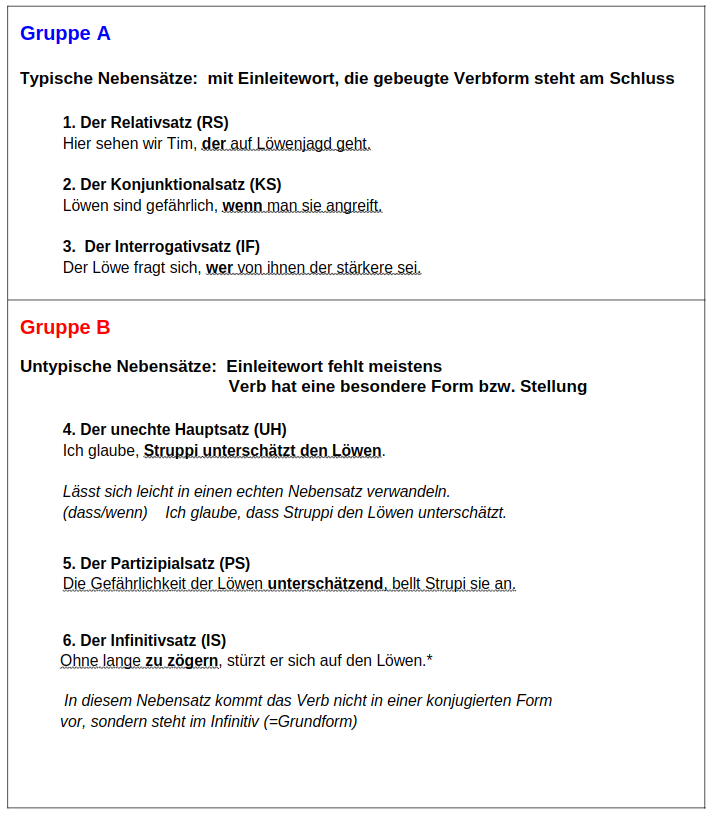
\includegraphics[width=\textwidth]{./german/imgs/nebensatz.png}

% TODO: Relativsatz al fa par da satzarten
\subsubsection{Relativsatz}

wird durch ein Relativpronomen eingeleitet: der, die, das; welcher, welche, welches, oder mit einem Relativadverb: wo, womit, wofür\\
\\
Der Mann, \textbf{derden Fernsehapparat repariert},\\
sagt zu der Frau, \textbf{die sich über den schlechten Empfang beklagthat}:\\
“Ich habe das Geräusch gefunden, \textbf{das Sie stört}“. 

\subsection{Stilistik}

\href{run:./includes/german/GBC/GBC_Stilistik_2023.pdf}{GBC\_Stilistik\_2023.pdf}

We use rhetorical figures to make the text more interesting.

\begin{description}
    \item[metaphor:] Break someone's hearth
    \item[Comparison:] He fights like a lion
    \item[gathering / Raffung:] He came, saw and conquered
    \item[paradox:] Life is death
    \item[inversion:] High is the Eiffel Tower
    \item[Citation:] "Did I ever tell you what the definition of insanity is? Insanity is doing the exact... same fucking thing... over and over again expecting... shit to change... That. Is. Crazy."\\ Michael Mando: Vaas Montenegro 
    \item[Cross position (chiasm):] One for all, all for one.
    \item[pleonasm:] She was personally present.
    \item[Sentence Fragment (Ellipse):] Nice!
    \item[oxymoron:] Loving hate:
    \item[Rhetorical question:] Am I insane?
    \item[irony:] A fire station burns down.
    \item[euphemism:] The release of employees.
    \item[alliteration:] Sally sells seashells by the sea shore.\\ How much wood could a woodchuck chuck if a woodchuck could chuck wood?
\end{description}